\documentclass[a4paper,11pt]{article}

\usepackage{pdp}

\usepackage{booktabs}
\usepackage{array}
\usepackage{amsmath}
\usepackage{amssymb}
\usepackage{enumitem}
\usepackage{caption}
\usepackage{subcaption}
\usepackage{float}
\usepackage{microtype}
\usepackage{csquotes}
\usepackage{xcolor}
\usepackage{tikz}
\usepackage{longtable}
\usepackage{tcolorbox}
\usepackage{mdframed}
\usepackage{minted}

%------------------------------------------------------------------------------
% INFOS
%------------------------------------------------------------------------------
\title{Shatranj --- Python}
\subtitle{Rapport final de projet de programmation}
\author{Benachour Souhila \\ Dries Amina \\ El Ghali Ayman \\ Marchoud Souhail \\ Meklat Sarah}

%------------------------------------------------------------------------------

\begin{document}

\maketitle
\thispagestyle{empty}

%==============================================================================
\section*{Introduction}
\addcontentsline{toc}{section}{Introduction}
%==============================================================================

Dans le cadre du cours de \emph{Projet de Programmation}, nous avons développé
\texttt{shatranj-python}, une implémentation complète du jeu de Shatranj en
Python~3.12. Le Shatranj est l'ancêtre direct des échecs modernes, né en Perse
sassanide aux \textsc{vi}\textsuperscript{e}--\textsc{vii}\textsuperscript{e}
siècles~\cite{Murray1913}~; ses règles de déplacement diffèrent sensiblement
des pièces actuelles, ce qui en fait un sujet de programmation à part entière.

Ce rapport présente les règles du jeu et leur contexte historique
(section~\ref{sec:regles}), les structures de données et algorithmes employés
(section~\ref{sec:algo}), l'architecture logicielle (section~\ref{sec:archi}),
puis détaille deux fonctionnalités clés~: l'intelligence artificielle
(section~\ref{sec:ia}) et l'interface graphique GTK (section~\ref{sec:gui}).
La section~\ref{sec:critique} dresse un bilan critique du projet.

%==============================================================================
\section{Explication détaillée du sujet}
\label{sec:regles}
%==============================================================================

\subsection{Contexte historique}

Le \emph{chaturanga} indien, attesté dès le \textsc{vi}\textsuperscript{e}
siècle~\cite{Murray1913}, est l'ancêtre commun de tous les jeux d'échecs
modernes. Il donna naissance au Shatranj en Perse sassanide~; ce jeu est
décrit en détail dans le \emph{Kit\=ab al-Shatr\=anj} d'al-Adl\={\i}~\cite{Murray1913},
traité du \textsc{ix}\textsuperscript{e} siècle qui codifie les règles, les
problèmes (\emph{mans\=ub\=at}) et les ouvertures. Le Shatranj se diffusa en
Europe médiévale et évolua vers les échecs modernes entre le
\textsc{xv}\textsuperscript{e} et le \textsc{xvi}\textsuperscript{e}
siècle~\cite{Shenk2006,Davidson1949}, notamment par l'acquisition par le Ferz
de la mobilité illimitée de la Dame moderne~\cite{Davidson1949}.

La différence la plus frappante concerne précisément ce \emph{Ferz}~: il ne
se déplace que d'une case en diagonale, là où la Dame moderne est la pièce la
plus puissante~\cite{Davidson1949}. L'Alfil, ancêtre du Fou, ne peut atteindre
que huit cases fixes toutes de même couleur~\cite{Browne2012}, contre une
diagonale entière pour le Fou actuel.

\subsection{Implémentations existantes}

\textbf{Fairy-Stockfish}~\cite{FairyStockfish} est un moteur d'échecs variants
basé sur Stockfish supportant le Shatranj via un système de pièces
configurables~; il utilise des bitboards 64~bits et l'algorithme NNUE.
La librairie \textbf{python-chess}~\cite{Pythonchess} permet de représenter
des variantes d'échecs en Python mais ne supporte pas nativement le Shatranj.
Notre implémentation se distingue par une interface graphique GTK~4 avec
horloge intégrée, deux thèmes de pièces SVG, un CLI complet avec historique
readline, et un moteur de règles spécifique au Shatranj (Bare King, promotion
uniquement en Ferz), sans dépendance externe pour le moteur de jeu.

\subsection{Le plateau et la notation}

Le Shatranj se joue sur un échiquier $8 \times 8$. Les colonnes sont désignées
par \texttt{a}--\texttt{h} et les rangées par \texttt{1}--\texttt{8}. En
interne, les cases sont numérotées de~0 (\texttt{a1}) à~63 (\texttt{h8})~:
\[
  \text{numéro} = \text{rangée} \times 8 + \text{colonne}
\]
\noindent\textbf{Exemple.} La case \texttt{e4}~: rangée~3, colonne~4,
numéro~$3 \times 8 + 4 = 28$.

\subsection{Les pièces et leurs déplacements}
Le jeu comporte six types de pièces. Les blanches sont notées en majuscules,
les noires en minuscules.

\begin{figure}[H]
\centering
% --- Ligne 1 : Shah, Ferz, Tour ---
\begin{minipage}[t]{0.30\textwidth}
  \centering
  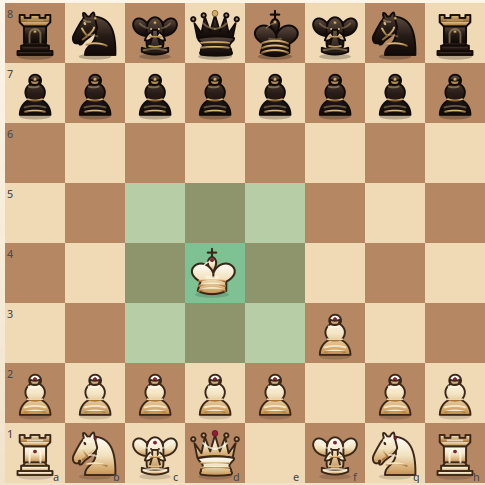
\includegraphics[width=0.65\textwidth]{shah.png}\\[0.4em]
  \textbf{Shah (K/k) --- Le Roi}\\[0.2em]
  \small Se déplace d'une case dans toutes les directions (horizontal, vertical,
  diagonal)~\cite{Murray1913}. C'est la pièce à protéger absolument~:
  si le Shah est mis en échec et mat, la partie est perdue.
\end{minipage}
\hfill
\begin{minipage}[t]{0.30\textwidth}
  \centering
  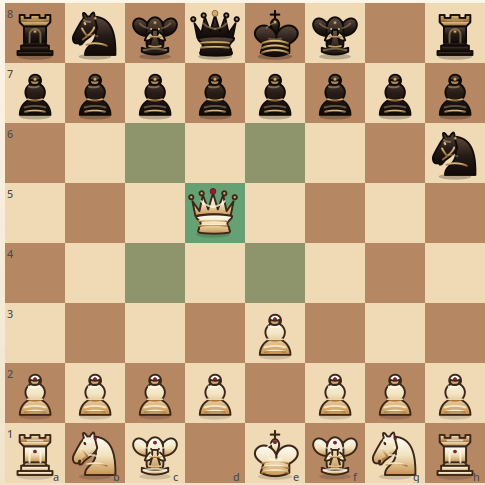
\includegraphics[width=0.65\textwidth]{ferz.png}\\[0.4em]
  \textbf{Ferz (F/f) --- Le Conseiller}\\[0.2em]
  \small Se déplace d'une \emph{seule} case en diagonale~\cite{Davidson1949}.
  C'est l'une des pièces les plus faibles du jeu.
\end{minipage}
\hfill
\begin{minipage}[t]{0.30\textwidth}
  \centering
  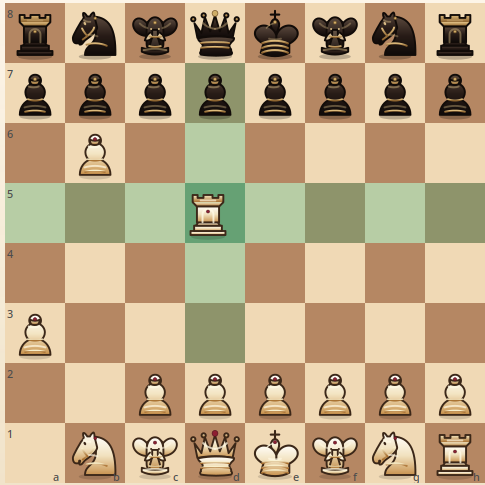
\includegraphics[width=0.65\textwidth]{tour.png}\\[0.4em]
  \textbf{Rook (R/r) --- La Tour}\\[0.2em]
  \small Se déplace en ligne droite (horizontale ou verticale) sur toute la
  longueur du plateau~\cite{Murray1913}. Bloquée par les pièces sur son chemin.
\end{minipage}

\vspace{1.5em}

% --- Ligne 2 : Alfil, Cavalier, Pion ---
\begin{minipage}[t]{0.30\textwidth}
  \centering
  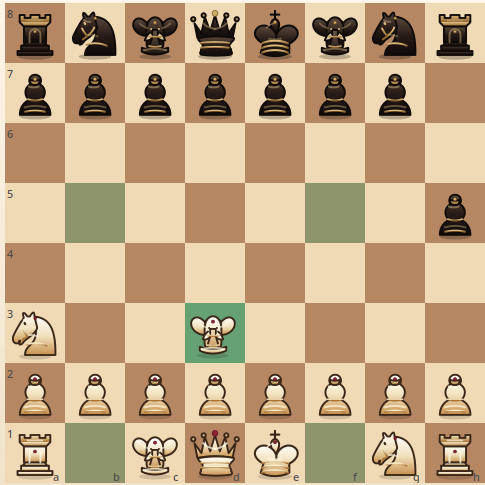
\includegraphics[width=0.65\textwidth]{alfil.png}\\[0.4em]
  \textbf{Alfil (A/a) --- L'Éléphant}\\[0.2em]
  \small Saute exactement deux cases en diagonale en franchissant la case
  intermédiaire~\cite{Browne2012}. Ne change jamais de couleur de case.
\end{minipage}
\hfill
\begin{minipage}[t]{0.30\textwidth}
  \centering
  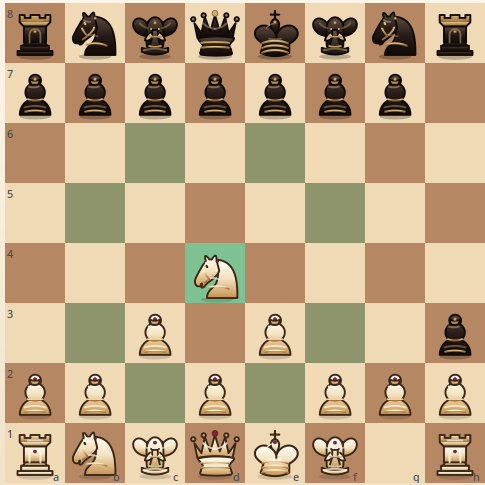
\includegraphics[width=0.65\textwidth]{cavalier.png}\\[0.4em]
  \textbf{Knight (N/n) --- Le Cavalier}\\[0.2em]
  \small Se déplace en \enquote{L}~: deux cases dans une direction puis une
  case perpendiculaire. Peut sauter par-dessus les autres pièces.
\end{minipage}
\hfill
\begin{minipage}[t]{0.30\textwidth}
  \centering
  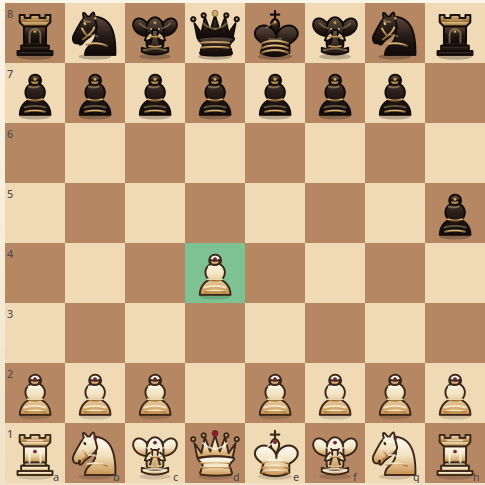
\includegraphics[width=0.65\textwidth]{pion.png}\\[0.4em]
  \textbf{Pawn (P/p) --- Le Pion}\\[0.2em]
  \small Avance d'une seule case vers l'avant. Capture en diagonale.
  Pas de double pas initial, ni de prise en passant.
  La promotion se fait uniquement en Ferz~\cite{Murray1913}.
\end{minipage}

\caption{Les six pièces du jeu et leurs déplacements}
\end{figure}

\subsection{Conditions de fin de partie}
\label{sec:finpartie}
Le Shatranj connaît trois conditions de fin de partie principales, dont deux
(\textbf{Pat} et \textbf{Bare King}) diffèrent fondamentalement des
échecs modernes.

\begin{figure}[H]
\centering
\begin{minipage}[t]{0.30\textwidth}
  \centering
  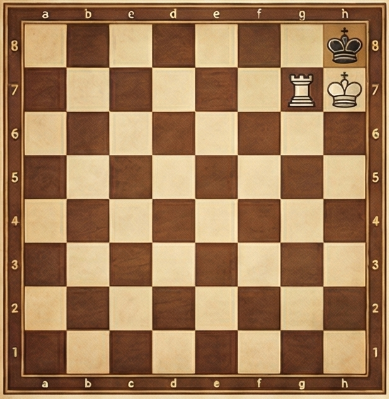
\includegraphics[width=\textwidth]{echec_et_mat.png}\\[0.4em]
  \textbf{Échec et mat}\\[0.2em]
  \small Le Shah adverse est en échec et ne peut s'échapper~:
  aucun coup légal ne le sort de la menace. Le joueur qui
  donne mat gagne immédiatement.
  \emph{(illustration générée par notebooklm)}
\end{minipage}
\hfill
\begin{minipage}[t]{0.30\textwidth}
  \centering
  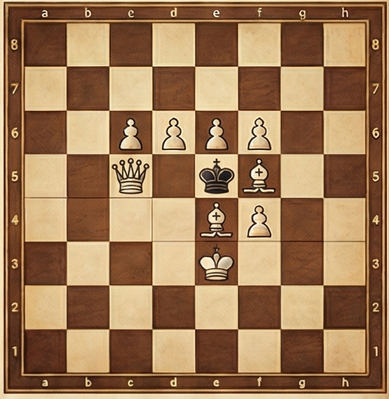
\includegraphics[width=\textwidth]{le_pat.png}\\[0.4em]
  \textbf{Pat --- Règle propre au Shatranj}\\[0.2em]
  \small Contrairement aux échecs modernes où le pat est nul, au Shatranj
  le joueur n'ayant aucun coup légal \textbf{perd} la partie~\cite{Murray1913,Davidson1949,Shenk2006}.
  \emph{(illustration générée par notebooklm)}
\end{minipage}
\hfill
\begin{minipage}[t]{0.30\textwidth}
  \centering
  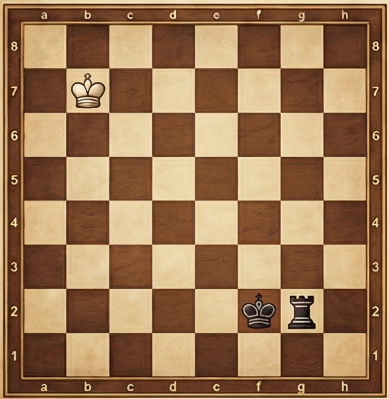
\includegraphics[width=\textwidth]{bare_king.png}\\[0.4em]
  \textbf{Bare King (\textit{Shah nu})}\\[0.2em]
  \small Si toutes les pièces d'un joueur sont capturées (seul son Shah reste),
  il perd immédiatement, même si ce Shah n'est pas en échec~\cite{Murray1913,Davidson1949,Shenk2006}.
  \emph{(illustration générée par notebooklm)}
\end{minipage}

\caption{Les trois conditions de fin de partie du Shatranj}
\end{figure}

\subsection{Analyse de la complexité du jeu}

Le facteur de branchement moyen est $b \approx 30$ (inférieur aux $\approx 35$
des échecs modernes car le Ferz et l'Alfil sont très limités). L'élagage
$\alpha$-$\beta$ ramène $b^d$ à $b^{d/2}$~\cite{Knuth1975,RussellNorvig2020}~:

\begin{center}
\begin{tabular}{lccc}
\toprule
Profondeur $d$ & Sans élagage ($30^d$) & Avec élagage ($30^{d/2}$) & Gain \\
\midrule
3 & 27\,000      & 164    & $\times 165$ \\
4 & 810\,000     & 900    & $\times 900$ \\
5 & 24\,300\,000 & 5\,477 & $\times 4\,437$ \\
\bottomrule
\end{tabular}
\end{center}

%==============================================================================
\section{Algorithmes et structures de données}
\label{sec:algo}
%==============================================================================

\subsection{Vue d'ensemble}

Le projet mobilise les structures et algorithmes suivants~:

\begin{itemize}[noitemsep]
  \item \textbf{Bitboards~:} entiers 64~bits représentant l'état du plateau~\cite{Shannon1950}.
  \item \textbf{AlphaBeta~:} Minimax optimisé, complexité $O(b^{d/2})$~\cite{Knuth1975}.
  \item \textbf{Iterative Deepening~:} approfondissement itératif avec limite de temps.
  \item \textbf{Zobrist hashing~:} hachage incrémental en $O(1)$~\cite{Zobrist1970}.
  \item \textbf{Table de transposition~:} mémoïsation des positions.
  \item \textbf{MCTS~:} recherche par simulations aléatoires~\cite{Browne2012}.
\end{itemize}

\subsection{Bitboards}

\subsubsection{Principe}

Un \emph{bitboard} est un entier non signé de 64~bits dans lequel chaque bit
représente une case du plateau~\cite{Shannon1950}. Le bit~$i$ vaut~1 si une
pièce donnée occupe la case~$i$. La classe \texttt{Board} maintient
12~bitboards ($6$~types de pièces $\times$ 2~couleurs).

\subsubsection{Numérotation des cases}

\begin{center}
\begin{tabular}{r|cccccccc}
  & a & b & c & d & e & f & g & h \\\hline
8 & 56 & 57 & 58 & 59 & 60 & 61 & 62 & 63 \\
7 & 48 & 49 & 50 & 51 & 52 & 53 & 54 & 55 \\
\vdots & \multicolumn{8}{c}{\dots} \\
2 &  8 &  9 & 10 & 11 & 12 & 13 & 14 & 15 \\
1 &  0 &  1 &  2 &  3 &  4 &  5 &  6 &  7 \\
\end{tabular}
\end{center}

\subsubsection{Implémentation Python~: spécificités et astuces}

En Python, les entiers sont de précision arbitraire~: il n'existe pas de type
\texttt{uint64} natif. Nous utilisons des entiers Python ordinaires et des
masques explicites lorsque nécessaire. Le module \texttt{data/bitboards/bitboard.py}
fournit les primitives avec validation systématique des indices via
\texttt{check\_square}~:

\begin{minted}[frame=single,fontsize=\small]{python}
def check_square(square: int) -> bool:
    if square < 0 or square >= NUM_SQUARES:   # NUM_SQUARES = 64
        raise InvalidSquareError(
            f"Square {square} must be in [0, {NUM_SQUARES - 1}]")
    return True

def set_bit_at(bitboard: int, square: int) -> int:
    check_square(square)
    return bitboard | (1 << square)

def clear_bit_at(bitboard: int, square: int) -> int:
    check_square(square)
    return bitboard & ~(1 << square)

def get_bit_at(bitboard: int, square: int) -> int:
    check_square(square)
    return (bitboard >> square) & 1

def count_bits(bitboard: int) -> int:
    return bitboard.bit_count()
\end{minted}

\paragraph{Astuce~: \texttt{bit\_count()} natif Python 3.10+.}
Plutôt que d'utiliser \texttt{bin(x).count('1')}, nous utilisons la méthode
\texttt{.bit\_count()} introduite en Python~3.10, qui délègue au compilateur
une instruction \texttt{popcount} optimisée sur les architectures modernes.
Le gain est significatif dans l'évaluateur qui compte les pièces à chaque nœud.

\paragraph{Astuce~: isolation du LSB en complément à deux.}
\begin{minted}[frame=single,fontsize=\small]{python}
def get_lsb(bitboard: int) -> int:
    if bitboard == 0:
        return -1
    return (bitboard & -bitboard).bit_length() - 1


def pop_lsb(bitboard: int) -> tuple[int, int]:
    idx = get_lsb(bitboard)
    if idx == -1:
        return -1, 0
    return idx, bitboard ^ (1 << idx)


def squares_from_bitboard(bitboard: int) -> list[int]:
    squares: list[int] = []
    bb = bitboard
    while bb:
        idx, bb = pop_lsb(bb)
        squares.append(idx)
    return squares
\end{minted}

$x \mathbin{\&} (-x)$ isole le bit le moins significatif en $O(1)$~: en
complément à deux, $-x = \lnot x + 1$, donc tous les bits inférieurs au
LSB sont mis à~0. \texttt{squares\_from\_bitboard} permet d'itérer sur toutes
les cases occupées en $O(k)$ où $k$ est le nombre de bits actifs.

\subsubsection{Application et annulation d'un coup en O(1)}

L'application d'un coup modifie exactement deux bits~: on efface la case source
et on active la case destination. En cas de capture, on efface en plus le bit
adverse. Ces opérations sont toutes en $O(1)$~:

\begin{minted}[frame=single,fontsize=\small]{python}
def apply_move(self, move: Move) -> tuple[str, str] | None:
        """Play a move and promote pawns reaching the last rank to ferz."""
        captured = self.get_piece_at(move.to_square)
        self.move_piece(move.from_square, move.to_square)
        if self._is_promotion_move(move):
            self.set_piece(FERZ, move.color, move.to_square)
        return captured

    def undo_move(self, move: Move, captured: tuple[str, str] | None) -> None:
        """Undo a move, including promotion moves explored by the AI."""
        self.clear_piece(move.to_square)
        self.set_piece(move.piece_type, move.color, move.from_square)
        if captured is not None:
            piece, color = captured
            self.set_piece(piece, color, move.to_square)
\end{minted}

\texttt{apply\_move} retourne la pièce capturée sous forme de tuple 
(type, couleur) ou None. \texttt{undo\_move} reçoit ce même tuple

\subsubsection{Génération des coups légaux}

\begin{minted}[frame=single,fontsize=\small]{python}
def generate_legal_moves(self, board: Board, color: str) -> list[Move]:
        legal = []
        for move in self.generate_pseudo_legal_moves(board, color):
            if not self.is_valid_move(board, move):
                continue
            captured = board.apply_move(move)  # joue le coup
            in_check = self._is_in_check(board, color)  # Shah en danger ?
            board.undo_move(move, captured)  # annule le coup
            if not in_check:
                legal.append(move)  # coup légal → on le garde
        return legal
\end{minted}

\noindent\textbf{Complexité.} Pour chaque coup pseudo-légal, \texttt{is\_in\_check} génère 
tous les coups adverses en parcourant les 64 cases pour chaque type de pièce, soit une complexité 
de $O(64 \times 6)$. 

Au total, la complexité est $O(M \times 384)$, où $M$ est le nombre de coups pseudo-légaux.
Avec $M \leq 100$ en pratique, cela reste négligeable par rapport aux nœuds explorés.

\subsection{AlphaBeta (Minimax avec élagage)}

L'algorithme Minimax~\cite{Shannon1950} modélise le jeu comme un arbre
alternant MAX (l'IA) et MIN (l'adversaire). L'élagage $\alpha$-$\beta$~\cite{Knuth1975}
l'améliore~: dès que $\beta \leq \alpha$, la branche est abandonnée.

\begin{minted}[frame=single,fontsize=\small]{python}
def _alphabeta(
        self,
        board: Board,
        depth: int,
        alpha: float,
        beta: float,
        is_maximizing: bool,
        ai_color: str,
        current_color: str,
        key: int,
    ) -> float:
        original_alpha = alpha
        # --- Transposition Table lookup ---
        tt_score, should_use = self._tt.get(key, depth, alpha, beta)
        if should_use:
            return tt_score
        # --- Base case: depth reached ---
        if depth == 0:
            return self._evaluator.evaluate(board, ai_color)
        legal_moves = self._engine.generate_legal_moves(board, current_color)
        # --- Base case: no moves ---
        if not legal_moves:
            if self._engine._is_in_check(board, current_color):
                return 9999.0 if not is_maximizing else -9999.0
            return 0.0
        opponent = BLACK if current_color == WHITE else WHITE
        if is_maximizing:
            best = float("-inf")
            for move in legal_moves:
                captured = board.apply_move(move)
                result_piece = board.get_piece_at(move.to_square)[0]
                captured_piece = captured[0] if captured else None
                captured_color = captured[1] if captured else None
                new_key = self._hasher.update_key(
                    key=key,
                    piece=move.piece_type,
                    color=current_color,
                    from_square=move.from_square,
                    to_square=move.to_square,
                    captured_piece=captured_piece,
                    captured_color=captured_color,
                    result_piece=result_piece,
                )
                score = self._alphabeta(
                    board=board,
                    depth=depth - 1,
                    alpha=alpha,
                    beta=beta,
                    is_maximizing=False,
                    ai_color=ai_color,
                    current_color=opponent,
                    key=new_key,
                )
                board.undo_move(move, captured)
                best = max(best, score)
                alpha = max(alpha, best)
                if beta <= alpha:
                    break  # beta cutoff
            # --- Store in Transposition Table ---
            if best <= original_alpha:
                flag = UPPER_BOUND
            if best >= beta:
                flag = LOWER_BOUND
            else:
                flag = EXACT
            self._tt.store(key, best, depth, flag)
            return best
        best = float("+inf")
        for move in legal_moves:
            captured = board.apply_move(move)
            result_piece = board.get_piece_at(move.to_square)[0]
            captured_color = current_color if captured else None
            new_key = self._hasher.update_key(
                key=key,
                piece=move.piece_type,
                color=current_color,def generate_legal_
                from_square=move.from_square,
                to_square=move.to_square,
                captured_piece=captured,
                captured_color=captured_color,
                result_piece=result_piece,
            )
            score = self._alphabeta(
                board=board,
                depth=depth - 1,
                alpha=alpha,
                beta=beta,
                is_maximizing=True,
                ai_color=ai_color,
                current_color=opponent,
                key=new_key,
            )
            board.undo_move(move, captured)
            best = min(best, score)
            beta = min(beta, best)
            if beta <= alpha:
                break  # alpha cutoff
        # --- Store in Transposition Table ---
        if best <= original_alpha:
            flag = UPPER_BOUND
        if best >= beta:
            flag = LOWER_BOUND
        else:
            flag = EXACT
        self._tt.store(key, best, depth, flag)
        return best

\end{minted}

\noindent\textbf{Déroulement.} Supposons $\alpha = 5$ (MAX a un coup valant~5).
Si MIN trouve~3 ($\beta = 3 \leq \alpha = 5$), cette branche est abandonnée~:
MAX ne la choisira jamais. À profondeur~4~: de $30^4 = 810\,000$ à
$\approx 900$~nœuds dans le meilleur cas~\cite{RussellNorvig2020}.

\subsection{Approfondissement itératif (Iterative Deepening)}

Plutôt que de chercher directement à profondeur~$d$, l'approfondissement
itératif explore successivement les profondeurs 1, 2, \ldots, $d$. L'avantage
principal est de toujours disposer d'un coup de repli si le temps s'écoule~:

\begin{minted}[frame=single,fontsize=\small]{python}
def best_move(self, board: Board, color: str) -> Move | None:    
        legal_moves = self._engine.generate_legal_moves(board, color)
        if not legal_moves:
            return None
        best_move = legal_moves[0]  # fallback: first legal move
        start_time = time.time()
        for current_depth in range(1, self._depth + 1):
            # check time limit before starting a new depth
            if self._time_limit is not None:
                elapsed = time.time() - start_time
                if elapsed >= self._time_limit:
                    break  # time is up → return best move from previous depth

            # search at current depth using Alpha-Beta
            self._ab._depth = current_depth
            move = self._ab.best_move(board, color)
            if move is not None:
                best_move = move  # update best move
            # check time limit after finishing a depth
            if self._time_limit is not None:
                if time.time() - start_time >= self._time_limit:
                    break
        return best_move
\end{minted}

\textbf{Avantage de l'ordonnancement des coups.} En théorie, la table de transposition pourrait 
conserver les résultats de profondeur $d{-}1$
pour guider l'ordonnancement à profondeur $d$.
Dans notre implémentation actuelle, la table est vidée au début de chaque appel à 
\texttt{best\_move}, ce qui limite cet avantage à l'intérieur d'une même profondeur.
Une amélioration future consisterait à ne pas vider la table entre les itérations.


%==============================================================================
\subsection{Hachage de Zobrist et table de transposition}
\label{sec:zobrist}
%==============================================================================

\subsubsection{Principe général et motivation}

Lors d'une recherche Alpha-Beta ou MCTS, le moteur explore des millions de
nœuds. Or, la même position peut être atteinte par des séquences de coups
différentes (\emph{transpositions})~: sans mémoïsation, ces positions seraient
réévaluées inutilement. La \textbf{table de transposition} (TT) cache
les résultats déjà calculés. Elle repose sur le \textbf{hachage de
Zobrist}~\cite{Zobrist1970}~: une méthode pour calculer
un identifiant unique (clé de 64 bits) pour chaque position du plateau.

\subsubsection{Construction de la table aléatoire}

Au démarrage, on génère \emph{une seule fois} un entier aléatoire de 64~bits
pour chaque triplet \texttt{(type\_pièce, couleur, case)}~:

\[
  \text{table}[\text{pièce}][\text{couleur}][\text{case}]
  \in \{0,\ldots,2^{64}-1\}
\]

Le nombre total d'entrées est $6 \times 2 \times 64 = 768$, auquel s'ajoute
un nombre aléatoire supplémentaire \texttt{black\_to\_move\_key} indiquant
quel joueur a le trait. On obtient ainsi 769 nombres aléatoires distincts.
Le générateur est initialisé avec la graine~42 pour garantir la
\textbf{reproductibilité} entre exécutions.

\begin{minted}[frame=single,fontsize=\small]{python}
# Initialisation (une seule fois à l'import du module)
rng = Random(42)
for piece in ALL_PIECES:            # 6 types
    for color in ALL_COLORS:        # 2 couleurs
        for square in range(64):    # 64 cases
            table[(piece, color, square)] = rng.getrandbits(64)
black_to_move_key = rng.getrandbits(64)
\end{minted}

\subsubsection{Calcul de la clé initiale et propriétés algébriques}

La clé d'une position est le \textbf{XOR} de tous les nombres aléatoires
correspondant aux pièces effectivement présentes sur le plateau~:

\[
  Z(\text{position}) = \bigoplus_{(p,c,s) \in \text{plateau}}
  \text{table}[p][c][s]
  \;\oplus\;
  \begin{cases}
    \texttt{black\_to\_move\_key} & \text{si c'est au tour des noirs} \\
    0 & \text{sinon}
  \end{cases}
\]

% Remplace le bloc tikzpicture de construction de la clé
\begin{figure}[H]
  \centering
  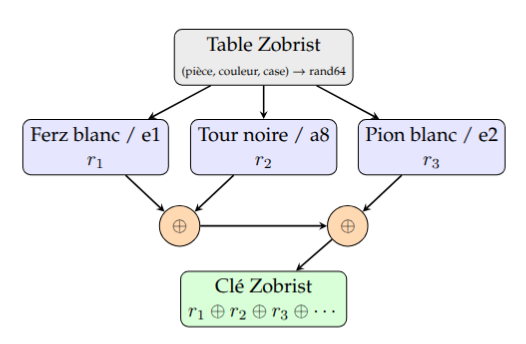
\includegraphics[width=0.82\textwidth]{constructionZ.png}
  \caption{Construction de la clé Zobrist par XOR des nombres aléatoires
  \emph{(illustration générée par chatGpt)}}
  \label{fig:zobrist}
\end{figure}


\subsubsection{Mise à jour incrémentale après un coup --- $O(1)$}

C'est ici que réside l'avantage décisif de Zobrist. Lorsqu'une pièce se déplace
de \texttt{from\_square} vers \texttt{to\_square}, la clé est mise à jour
avec \textbf{au maximum 3 XOR}~:

\noindent\textbf{Comparaison avec un hachage naïf.}
Un hachage naïf (ex.~\texttt{hash(str(board))}) nécessiterait de parcourir
les 64~cases à chaque nœud~: $O(64) = O(1)$ mais avec une constante 64 fois
plus grande. À profondeur~4, l'algorithme explore $\approx 900$~nœuds~;
l'économie est d'environ $900 \times 62 = 55\,800$ opérations par appel.

\paragraph{Undo en $O(1)$.} La propriété auto-inverse du XOR garantit que
\texttt{undo\_move} restaure la clé sans recalcul~: il suffit de rejouer les
mêmes XOR dans le même ordre.

\subsubsection{Probabilité de collision}

Deux positions différentes pourraient théoriquement produire la même clé de
64~bits (\emph{faux positif}). La probabilité est~:

\[
  P(\text{collision}) \approx \frac{1}{2^{64}} \approx 5.4 \times 10^{-20}
\]

Avec un million de positions en mémoire, la probabilité qu'une paire quelconque
entre en collision reste inférieure à $\sim 10^{-8}$. En pratique, les
collisions Zobrist n'ont jamais été observées et n'affectent pas la jouabilité.

\subsubsection{Structure de la table de transposition}

La TT associe chaque clé Zobrist à un triplet \textbf{(score, profondeur, flag)}~:

\begin{figure}[H]
  \centering
  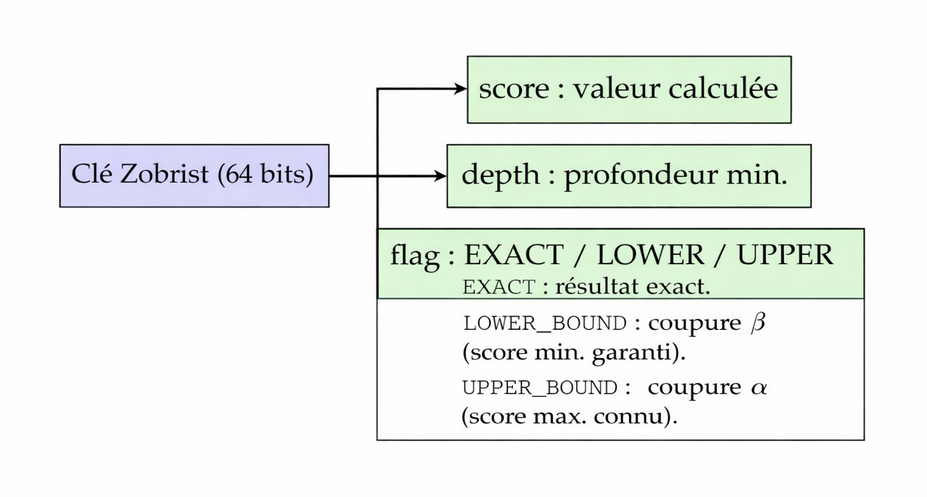
\includegraphics[width=0.75\textwidth]{entreTransposition.png}
  \caption{Structure d'une entrée dans la table de transposition
  \emph{(illustration générée par ChatGpt)}}
  \label{fig:tt-entry}
\end{figure}

\subsubsection{Consultation et mise à jour dans AlphaBeta}

\begin{minted}[frame=single,fontsize=\small]{python}
# --- Consultation de la TT au début de chaque nœud ---
def get(self, key: int, depth: int, alpha: float, beta: float):
        entry = self._table.get(key)
        if entry is None:
            return None, False
        # only use entries evaluated at sufficient depth
        if entry["depth"] < depth:
            return None, False
        score = entry["score"]
        flag = entry["flag"]
        if flag == EXACT:
            return score, True
        if flag == LOWER_BOUND and score >= beta:
            return score, True
        if flag == UPPER_BOUND and score <= alpha:
            return score, True
        return None, False
\end{minted}

\subsubsection{Politique de remplacement et partage entre algorithmes}

La TT est limitée à \textbf{10\,000 entrées} avec la stratégie
\emph{always-replace}~: si la table est pleine, la nouvelle entrée remplace
simplement l'ancienne. Cette politique favorise les positions récemment vues,
ce qui est cohérent avec l'approfondissement itératif.
Chaque algorithme (AlphaBeta, Iterative Deepening, MCTS) instancie sa propre table de transposition.
La table est vidée au début de chaque appel à \texttt{best\_move} afin d'éviter des résultats obsolètes
entre deux coups. Les bénéfices de la TT s'appliquent donc à l'intérieur d'une recherche unique, pour
les positions transposées rencontrées au cours de cette même recherche.
Sur les positions transposées rencontrées au cours d'une même recherche,
la TT réduit le nombre de nœuds évalués de \textbf{30 à 50\,\%}.

\subsubsection{Synthèse des propriétés Zobrist}

\begin{center}
\renewcommand{\arraystretch}{1.3}
\begin{tabular}{lll}
\toprule
\textbf{Propriété} & \textbf{Valeur / Comportement} & \textbf{Impact} \\
\midrule
Complexité calcul initial & $O(64)$ à la création du plateau & Fait une seule fois \\
Mise à jour après coup    & $O(1)$ (2--3 XOR) & Critique en recherche \\
Undo                      & $O(1)$ (mêmes XOR) & Symétrique \\
Taille de la table        & 769 entiers 64 bits $\approx$ 6~Ko & Négligeable \\
Probabilité de collision  & $\approx 5\times 10^{-20}$ & Ignorable \\
Reproductibilité          & Graine fixe = 42 & Débogage facilité \\
Portée & Par recherche (table vidée entre les coups) & Évite les résultats obsolètes\\
\bottomrule
\end{tabular}
\end{center}

%==============================================================================
\section{Architecture logicielle}
\label{sec:archi}
%==============================================================================

\subsection{Principe N-tiers}

L'application suit une architecture en couches strictement séparées~\cite{Fowler2002}
où chaque couche ne communique qu'avec la couche immédiatement inférieure.
La figure~\ref{fig:flux} illustre les trois couches.

La \textbf{couche Présentation} regroupe le CLI et le GUI GTK~4~: elle ne
contient aucune règle de jeu. La \textbf{couche Métier} (Domain) est le cœur
du programme~: moteur de règles, algorithmes d'IA, gestion de l'état via les
bitboards.

La \textbf{couche Présentation} regroupe le CLI et le GUI GTK~4~: elle ne
contient aucune règle de jeu. La \textbf{couche Métier} (Domain) est le cœur
du programme~: moteur de règles, algorithmes d'IA, gestion de l'état via les
bitboards. La \textbf{couche Données} gère la persistance (format texte ASCII)
et les primitives bit-à-bit.

\subsection{Flux d'interactions}

\begin{figure}[H]
  \centering
  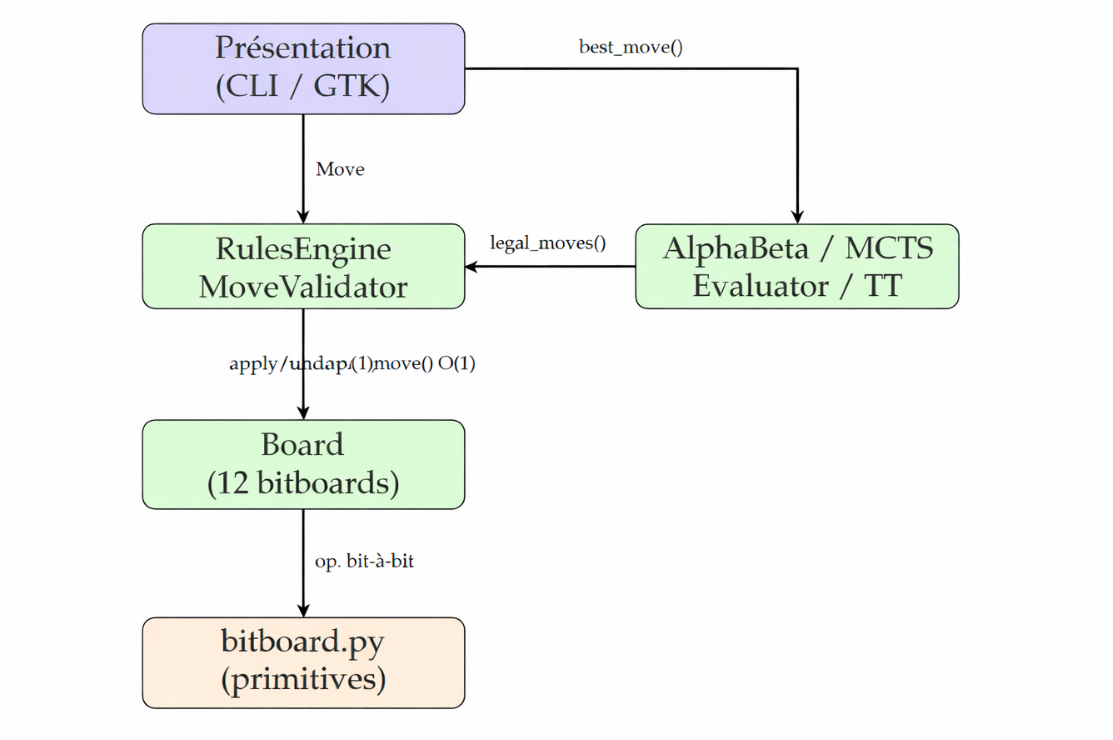
\includegraphics[width=0.82\textwidth]{diagramme d'interaction.png}
  \caption{Flux d'interaction entre les couches
  \emph{(illustration générée par ChatGpt)}}
  \label{fig:flux}
\end{figure}

Lorsqu'un utilisateur joue un coup (CLI ou GUI), la couche Présentation
construit un objet \texttt{Move} et le transmet au \texttt{RulesEngine}.
Celui-ci vérifie la légalité via \texttt{MoveValidator}, puis appelle
\texttt{Board.apply\_move()} qui modifie les bitboards en $O(1)$. Pour l'IA,
\texttt{AIPlayer.choose\_move()} sélectionne l'algorithme configuré (AlphaBeta, Iterative
Deepening ou MCTS),lequel gère en interne sa propre table de transposition, et renvoie le
meilleur coup.Dans le GUI, l'IA s'exécute dans un thread dédié afin de ne pas bloquer l'interface.

%------------------------------------------------------------------------------
\subsection{Principales interfaces entre couches --- Schéma d'API}
\label{sec:interfaces}
%------------------------------------------------------------------------------

Plutôt qu'une liste textuelle, le schéma ci-dessous représente les quatre
interfaces contractuelles entre les couches, avec la direction du flux de
données et les types échangés.

\begin{figure}[H]
  \centering
  \includegraphics[width=\textwidth]{interaction_interface.png}
  \caption{Schéma des interfaces contractuelles entre les trois couches
  \emph{(illustration réalisée par les auteurs sous Figma)}}
  \label{fig:interfaces}
\end{figure}

\noindent\textbf{Lecture du schéma.}
Les flèches pleines ($\to$) indiquent le sens de l'appel~; les flèches
($\dashleftarrow$) indiquent le retour de valeur. Chaque couche
n'est autorisée à importer que les symboles de la couche inférieure, ce qui
garantit une séparation des responsabilités stricte et facilite les tests
unitaires.

%==============================================================================
\section{Fonctionnalité approfondie~1 : Intelligence Artificielle}
\label{sec:ia}
%==============================================================================

\subsection{Vue d'ensemble}

Le module \texttt{domain/ai/} propose quatre algorithmes~:
\texttt{AlphaBeta} (profondeur~4), \texttt{Minimax} basique,
\texttt{IterativeDeepening} (profondeur~4 avec limite de temps) et
\texttt{MCTS} (500~simulations par coup). Tous partagent le même
\texttt{Evaluator}.

\subsection{Fonction d'évaluation}

L'\texttt{Evaluator} propose trois niveaux~:
\begin{enumerate}[noitemsep]
  \item \textbf{Material~:} somme algébrique des valeurs (Pion=1,
    Alfil=Ferz=2, Cavalier=6, Tour=9)~.
  \item \textbf{Positional~:} material + bonus positionnel par table de
    64~valeurs pour chaque type de pièce~; tables miroirs pour les noirs.
  \item \textbf{Advanced~:} positional + mobilité (nombre de coups légaux),
    contrôle du centre (+2~pts pour d4/e4/d5/e5), sécurité du Shah (malus
    si proche du centre).
\end{enumerate}

\subsection{Monte Carlo Tree Search (MCTS)}

\subsubsection{Principe et schéma}

\begin{figure}[H]
  \centering
  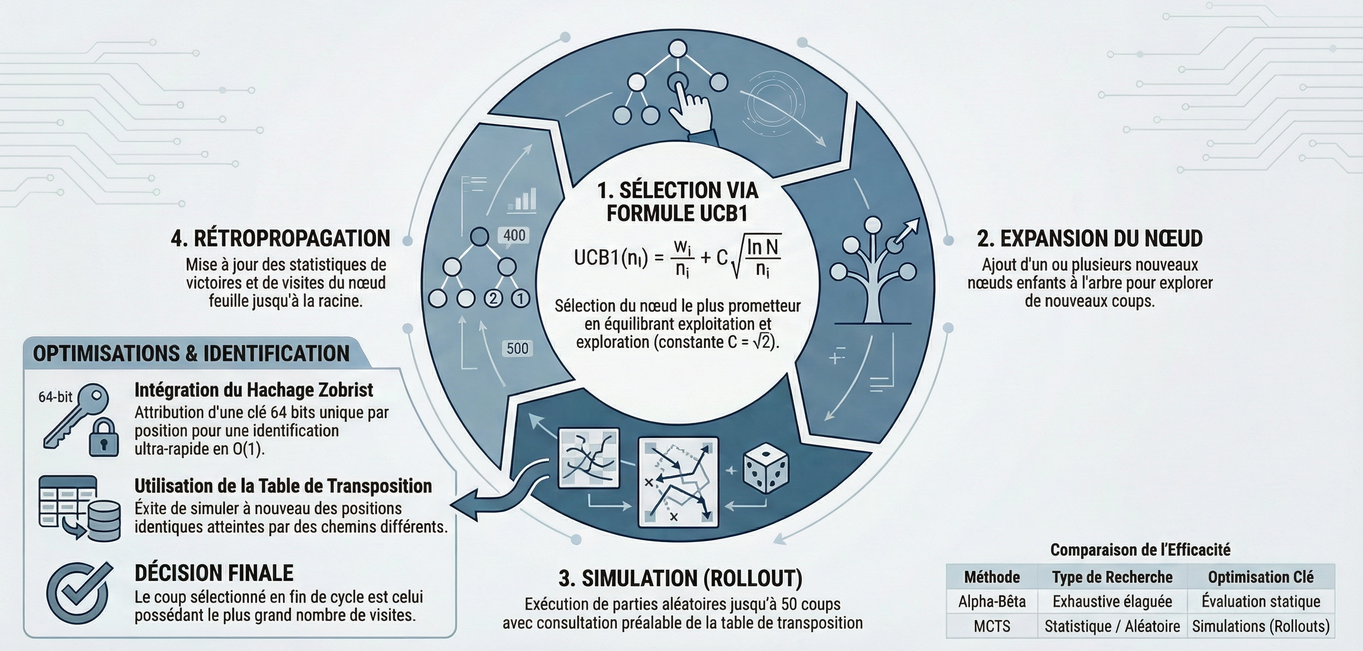
\includegraphics[width=0.82\textwidth]{mcts.png}
  \caption{Les quatre phases du MCTS~: sélection, expansion, simulation,
           rétropropagation~\cite{Browne2012}
           \emph{(illustration générée par notebooklm)}}
  \label{fig:mcts}
\end{figure}

Le MCTS~\cite{Browne2012} évalue les positions par simulations aléatoires.
À la différence d'AlphaBeta qui nécessite une fonction d'évaluation statique,
le MCTS tire sa force de l'accumulation de milliers de parties simulées.

\subsubsection{Structure MCTSNode}

Chaque nœud de l'arbre conserve les statistiques nécessaires à UCB1~:

\begin{minted}[frame=single,fontsize=\small]{python}
class MCTSNode:
    def __init__(
        self,
        move: Move | None,
        parent: "MCTSNode | None",
        color: str,
    ) -> None:
        self.move = move
        self.parent = parent
        self.color = color
        self.children: list["MCTSNode"] = []
        self.wins: float = 0.0
        self.visits: int = 0
        self.untried: list[Move] = []
    def is_fully_expanded(self) -> bool:
        """Return True if all moves have been explored."""
        return len(self.untried) == 0
\end{minted}

\subsubsection{Formule UCB1 et sélection}

\[
  \text{UCB1}(n_i) = \frac{w_i}{n_i} + C\sqrt{\frac{\ln N}{n_i}},
  \quad C = \sqrt{2}
\]

Le terme $\frac{w_i}{n_i}$ favorise l'\emph{exploitation} des bons nœuds~;
$C\sqrt{\frac{\ln N}{n_i}}$ favorise l'\emph{exploration} des nœuds peu visités.

\begin{minted}[frame=single,fontsize=\small]{python}
def best_child(self, exploration: float = 1.41) -> "MCTSNode":
        return max(
            self.children,
            key=lambda c: (c.wins / c.visits)
            + exploration * math.sqrt(math.log(self.visits) / c.visits),
        )
\end{minted}

\subsubsection{Rollout avec table de transposition}

Notre MCTS intègre la table de transposition dans la phase de simulation~:
avant de lancer un rollout aléatoire, on consulte la TT pour éviter de
rejouer des positions déjà connues~:

\begin{minted}[frame=single,fontsize=\small]{python}

    def _rollout(
        self,
        board: Board,
        current_color: str,
        ai_color: str,
        max_moves: int = 50,
    ) -> float:
        color = current_color
        # check TT for this position
        key = self._hasher.compute_key(board, color)
        tt_score, should_use = self._tt.get(key, 0, float("-inf"), float("+inf"))
        if should_use:
            return tt_score
        for _ in range(max_moves):
            legal_moves = self._engine.generate_legal_moves(board, color)
            # no moves -> checkmate or stalemate
            if not legal_moves:
                if self._engine._is_in_check(board, color):
                    opponent = BLACK if color == WHITE else WHITE
                    result = 1.0 if opponent == ai_color else 0.0
                else:
                    result = 0.5
                self._tt.store(key, result, 0, EXACT)
                return result
            # bare king -> opponent wins
            if self._engine.is_bare_king(board, color):
                opponent = BLACK if color == WHITE else WHITE
                result = 1.0 if opponent == ai_color else 0.0
                self._tt.store(key, result, 0, EXACT)
                return result
            # play a random move
            move = random.choice(legal_moves)
            board.apply_move(move)
            color = BLACK if color == WHITE else WHITE
        # move limit reached -> draw
        self._tt.store(key, 0.5, 0, EXACT)
        return 0.5
        \end{minted}

\noindent
À partir du nœud nouvellement créé, une partie aléatoire est simulée jusqu'à
l'obtention d'un état terminal ou jusqu'à la limite de \texttt{max\_moves}
coups. À chaque tour, un coup légal est choisi uniformément au hasard parmi
tous les coups disponibles. Le résultat est encodé~: 1,01{,}0
1,0 si l'IA gagne (mat adverse ou Bare King), 0,00{,}0
0,0 si elle perd, 0,50{,}5
0,5 en cas de position nulle. Le pat --- aucun coup légal sans être en échec 
--- est traité comme un résultat nul (0,50{,}5
0,5) dans le MCTS, car la simulation ne peut pas déterminer avec certitude 
qui a provoqué le pat. Ce traitement diverge légèrement de la règle officielle 
(section~\ref{sec:finpartie}) et constitue une limite connue de notre implémentation MCTS.
Avant de simuler, la position est indexée par sa clé de Zobrist~: si elle
a déjà été simulée, le résultat mis en cache est retourné immédiatement,
évitant ainsi des parties redondantes.

\subsubsection{Rétropropagation et choix final}

\begin{minted}[frame=single,fontsize=\small]{python}
def _backpropagate(self, node: "MCTSNode", result: float) -> None:

        while node is not None:
            node.visits += 1
            node.wins += result
            result = 1.0 - result
            node = node.parent
\end{minted}

\noindent
Le résultat $r \in \{0{,}0\;;\;0{,}5\;;\;1{,}0\}$ est propagé du nœud
feuille jusqu'à la racine en remontant la chaîne de parents. À chaque nœud,
\texttt{visits} est incrémenté de~$1$ et \texttt{wins} augmenté de~$r$.
La valeur est ensuite \emph{inversée} ($r \leftarrow 1 - r$) avant de
passer au nœud parent~: une victoire pour le fils est une défaite pour le
père, garantissant ainsi la cohérence de la formule UCB1 à tous les niveaux
de l'arbre.

\noindent
Le coup final retenu est le plus \emph{visité} (non le meilleur ratio
victoires/visites)~: la fréquence de visite est un indicateur plus
robuste~\cite{Browne2012}. Le MCTS utilise également une copie légère du
plateau pour chaque simulation (\texttt{\_copy\_board} copie uniquement
le dictionnaire de bitboards), ce qui évite les copies profondes coûteuses.

\begin{figure}[H]
  \centering
  \includegraphics[width=\textwidth]{exemple_mcts.png}
  \caption{Illustration du MCTS~: exploration asymétrique, simulation aléatoire
  et algorithme \textit{anytime}, comparés au Minimax classique.
  \emph{(illustration générée par notebooklm)}}
  \label{fig:mcts_exemple}
\end{figure}

%==============================================================================
\section{Fonctionnalité approfondie~2 : Interface graphique GTK~4}
\label{sec:gui}
%==============================================================================

\subsection{Vue d'ensemble}

L'interface graphique est réalisée avec \textbf{PyGObject}~\cite{Pythonchess},
le binding Python de GTK~4. Elle reproduit toutes les fonctionnalités du CLI
dans une fenêtre visuelle~: nouvelle partie avec dialogue de configuration,
horloge intégrée (Bullet/Blitz/Rapid/Custom), undo/redo, sauvegarde,
hint, mode IA avec thread dédié.


\subsection{Architecture du widget plateau}

Le widget \texttt{BoardWidget} hérite de \texttt{Gtk.DrawingArea} et utilise
\textbf{Cairo} pour le rendu et \textbf{librsvg} (\texttt{Rsvg.Handle})
pour charger les pièces au format SVG~:

\begin{minted}[frame=single,fontsize=\small]{python}
class BoardWidget(Gtk.DrawingArea):
 def __init__(self, engine: RulesEngine) -> None:
        super().__init__()
        self._engine = engine
        self._board: Board | None = None
        self._current_color: str = WHITE
        self._interaction_enabled: bool = True
        self._flipped: bool = False
        # Click-to-move state
        self._selected_square: int | None = None
        self._valid_moves: list[Move] = []
        # Drag'n'drop state
        self._drag_square: int | None = None
        self._drag_x: float = 0.0
        self._drag_y: float = 0.0
        self._dragging: bool = False
        # Callback called when a move is played: fn(move: Move)
        self.on_move_played = None
        # Load SVG piece images
        self._pieces = self._load_pieces()
        # Drawing
        self.set_draw_func(self._draw)
        # Click handler (click-to-move)
        click = Gtk.GestureClick.new()
        click.connect("pressed", self._on_click)
        self.add_controller(click)
        # Drag handler (drag'n'drop)
        drag = Gtk.GestureDrag.new()
        drag.connect("drag-begin", self._on_drag_begin)
        drag.connect("drag-update", self._on_drag_update)
        drag.connect("drag-end", self._on_drag_end)
        self.add_controller(drag)
\end{minted}

\subsubsection{Dialogue de configuration}

\begin{figure}[H]
  \centering
  \fbox{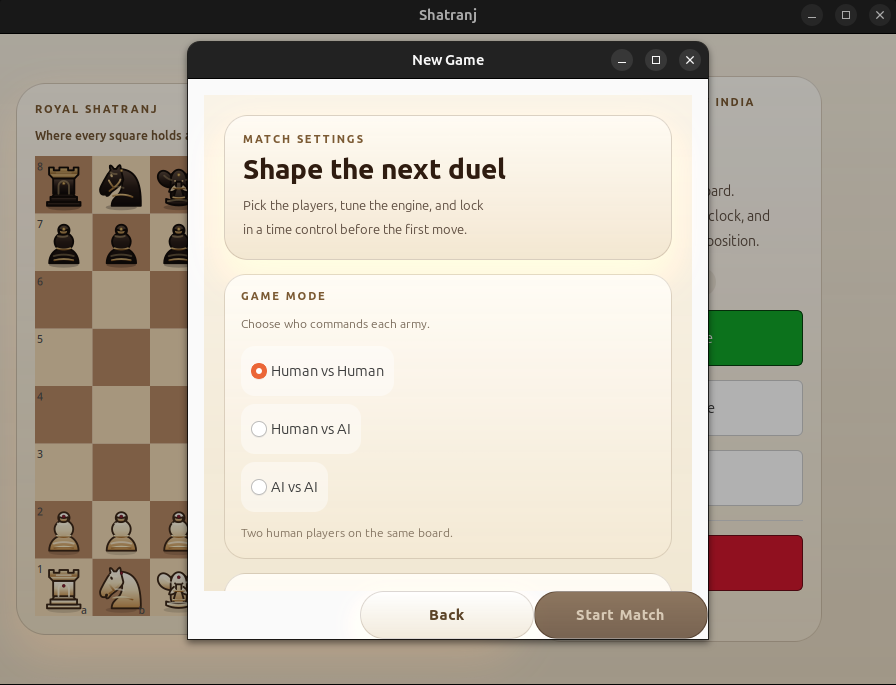
\includegraphics[width=0.75\textwidth]{GUI_SCREENSHOT_MENU.png}}
  \caption{Dialogue de configuration d'une nouvelle partie}
  \label{fig:gui_menu}
\end{figure}

\subsubsection{Rendu Cairo + SVG vectoriel}

Chaque pièce est chargée une seule fois via \texttt{Rsvg.Handle.new\_from\_file()}
et mise en cache dans \texttt{self.\_pieces}. Le rendu à l'écran utilise
\texttt{handle.render\_cairo(cr)} après une transformation de coordonnées
(translation + échelle). Le scaling est calculé dynamiquement depuis la taille
du widget~:

\begin{minted}[frame=single,fontsize=\small]{python}
def _board_geometry(width: int, height: int) -> tuple[float, float, float]:
    board_size = min(width, height)
    square_size = board_size / BOARD_SIZE
    offset_x = (width - board_size) / 2
    offset_y = (height - board_size) / 2
    return square_size, offset_x, offset_y
\end{minted}

Ce calcul garantit que le plateau reste carré et centré quelle que soit la
taille de la fenêtre. Les pièces sont mises à l'échelle dynamiquement~:

\begin{minted}[frame=single,fontsize=\small]{python}
has_size, svg_w, svg_h = handle.get_intrinsic_size_in_pixels()
            if not has_size or svg_w == 0 or svg_h == 0:
                svg_w, svg_h = 45.0, 45.0
            scale = sq / max(svg_w, svg_h)
            cr.save()
            cr.translate(x, y)
            cr.scale(scale, scale)
            handle.render_cairo(cr)
            cr.restore()
\end{minted}

La formule \texttt{scale = sq / max(svg\_w, svg\_h)} assure que quelle que
soit la taille intrinsèque du SVG (45×45, 128×128, etc.), la pièce occupe
\emph{exactement} une case. Toutes les pièces ont ainsi des dimensions
\textbf{identiques} à l'écran, ce qui garantit un rendu cohérent et
visuellement propre.

\paragraph{Deux thèmes de pièces.}
Le widget sélectionne automatiquement le thème \texttt{pieces\_royal/} s'il
existe, et se replie sur \texttt{pieces/} sinon. Les SVG utilisent la notation
standard~: \texttt{wK.svg} (Shah blanc), \texttt{bA.svg} (Alfil noir), etc.

\begin{figure}[H]
  \centering
  \fbox{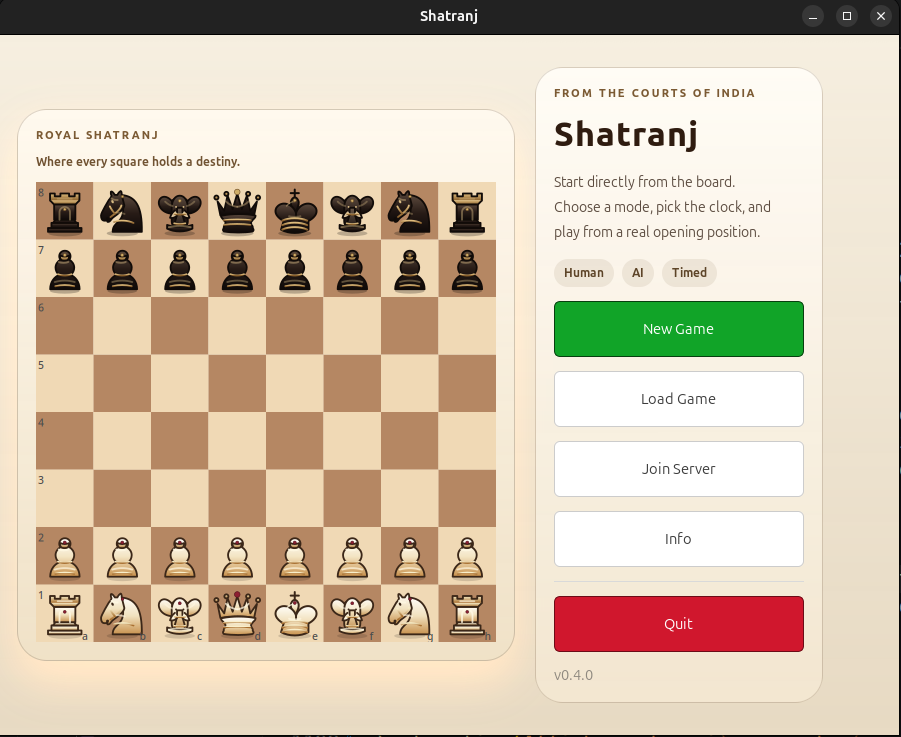
\includegraphics[width=0.75\textwidth]{GUI_SCREENSHOT_BOARD.png}}
  \caption{Plateau avec pièces SVG (thème Royal)}
  \label{fig:gui_board}
\end{figure}

%----------------------------------------------------------------------
\subsection{Affichage des pièces capturées --- Détail technique}
\label{sec:captures}
%----------------------------------------------------------------------

\subsubsection{Architecture des bandeaux de captures}

Les pièces capturées sont affichées dans deux \textbf{strips horizontaux}
(bandeaux) positionnés respectivement au-dessus et en dessous du plateau.
Le strip du haut affiche les pièces blanches capturées par les noirs~; celui
du bas affiche les pièces noires capturées par les blancs.


\subsubsection{Implémentation --- De l'historique aux icônes}

La logique de calcul des captures est scindée en deux fonctions~:

\paragraph{Méthode primaire~: \texttt{\_captured\_pieces\_from\_history}.}
Cette méthode parcourt la liste des coups joués (\texttt{state.get\_history()})
et collecte chaque pièce dont \texttt{move.captured\_piece} est non nul.
Elle est fiable car elle reflète exactement le déroulement de la partie,
y compris après un undo/redo~:

\begin{minted}[frame=single,fontsize=\small]{python}
def _captured_pieces_from_history(history) -> dict[str, list[str]] | None:
    captured = {
        WHITE: [],
        BLACK: [],
    }
    for move in history:
        if not move.captured_piece:
            continue
        if move.captured_piece not in STARTING_PIECE_COUNTS:
            return None
        captured_color = BLACK if move.color == WHITE else WHITE
        captured[captured_color].append(move.captured_piece)
    return {
        color: _sort_captured_piece_types(captured[color]) for color in (WHITE, BLACK)
    }
\end{minted}

\paragraph{Méthode de repli~: \texttt{\_captured\_pieces\_from\_board}.}
Pour les sauvegardes anciennes dont l'historique ne contient pas les captures,
on déduit les pièces manquantes en comparant le nombre de pièces sur le
plateau avec les effectifs de départ~:

\begin{minted}[frame=single,fontsize=\small]{python}
STARTING_PIECE_COUNTS = {FERZ: 1, ROOK: 2, ALFIL: 2, KNIGHT: 2, PAWN: 8}

def _captured_pieces_from_board(board) -> dict[str, list[str]]:
    """Fallback capture view for legacy saves without capture detail."""
    remaining = {
        WHITE: {piece: 0 for piece in STARTING_PIECE_COUNTS},
        BLACK: {piece: 0 for piece in STARTING_PIECE_COUNTS},
    }
    for square in range(64):
        piece_info = board.get_piece_at(square)
        if piece_info is None:
            continue

        piece, color = piece_info
        if piece in STARTING_PIECE_COUNTS:
            remaining[color][piece] += 1
    captured = {
        WHITE: [],
        BLACK: [],
    }
    for color in (WHITE, BLACK):
        for piece in CAPTURE_DISPLAY_ORDER:
            missing = STARTING_PIECE_COUNTS[piece] - remaining[color][piece]
            captured[color].extend([piece] * max(0, missing))
    return captured
\end{minted}

\paragraph{Affichage --- \texttt{\_make\_captured\_piece\_widget}.}
Chaque pièce capturée est représentée par une icône de \textbf{20×20 pixels}
(taille fixe), construite depuis le même fichier SVG que le plateau~:

\begin{minted}[frame=single,fontsize=\small]{python}
def _make_captured_piece_widget(self, piece: str, color: str):
        """Build one small piece icon for the capture strips."""
        path = get_piece_asset_path(piece, color)
        if path is not None:
            picture = Gtk.Picture.new_for_filename(path)
            picture.set_size_request(20, 20)
            if hasattr(picture, "set_can_shrink"):
                picture.set_can_shrink(True)
            if hasattr(picture, "set_keep_aspect_ratio"):
                picture.set_keep_aspect_ratio(True)
            picture.set_tooltip_text(PIECE_LABELS.get(piece, piece.title()))
            return picture

        label = Gtk.Label(label=piece[:1].upper())
        label.set_halign(Gtk.Align.CENTER)
        label.set_valign(Gtk.Align.CENTER)
        label.set_tooltip_text(PIECE_LABELS.get(piece, piece.title()))
        return label
\end{minted}

\textbf{Point clé --- Cohérence des dimensions.}
La taille de 20×20 est choisie pour que les captures restent discrètes
et ne rivalisent pas visuellement avec le plateau. La méthode
\texttt{set\_keep\_aspect\_ratio(True)} garantit que les SVG de formes
variées (pion court, tour large) ne sont jamais déformés~; la méthode
\texttt{set\_can\_shrink(True)} permet à GTK de réduire l'image si l'espace
devient insuffisant. Ces deux appels combinent le même principe que sur le
plateau (\texttt{scale = sq / max(svg\_w, svg\_h)}) mais délèguent le calcul
à GTK plutôt qu'à Cairo.

\paragraph{Rafraîchissement.}
\texttt{\_update\_captured\_pieces()} est appelée systématiquement depuis
\texttt{\_refresh\_game\_view()} après chaque coup, undo ou chargement.
Elle vide d'abord les strips (\texttt{\_clear\_box\_children}) puis les
remplit avec les nouvelles icônes~:

\begin{minted}[frame=single,fontsize=\small]{python}
def _update_captured_pieces(self) -> None:
        """Refresh the captured-piece strips above and below the board."""
        if not hasattr(self, "_black_capture_strip"):
            return
        captured = _captured_pieces_for_display(self._state)
        top_color, bottom_color = _captured_piece_colors_for_display(
            self._network_my_color
        )
        for captured_color, strip in (
            (top_color, self._black_capture_strip),
            (bottom_color, self._white_capture_strip),
        ):
            self._clear_box_children(strip)
            for piece in captured[captured_color]:
                strip.append(self._make_captured_piece_widget(piece, captured_color))
\end{minted}

\subsubsection{Ordre d'affichage des captures}

Les pièces ne sont pas affichées dans l'ordre de capture chronologique mais
dans un \textbf{ordre visuel stable}~: Tour $>$ Cavalier $>$ Alfil $>$
Ferz $>$ Pion. Cet ordre (défini par \texttt{CAPTURE\_DISPLAY\_ORDER}) est
identique à celui utilisé dans les clients d'échecs modernes et rend le bandeau
lisible d'un coup d'œil.

\begin{center}
\renewcommand{\arraystretch}{1.3}
\begin{tabular}{lcccc}
\toprule
\textbf{Pièce} & \textbf{Position} & \textbf{SVG source} & \textbf{Taille icône} & \textbf{Tooltip} \\
\midrule
Tour  (Rook)   & 1 (gauche) & \texttt{wR.svg / bR.svg} & 20×20 px & ``Rook''   \\
Cavalier (Knight) & 2        & \texttt{wN.svg / bN.svg} & 20×20 px & ``Knight'' \\
Alfil          & 3          & \texttt{wA.svg / bA.svg} & 20×20 px & ``Alfil''  \\
Ferz           & 4          & \texttt{wF.svg / bF.svg} & 20×20 px & ``Ferz''   \\
Pion  (Pawn)   & 5 (droite) & \texttt{wP.svg / bP.svg} & 20×20 px & ``Pawn''   \\
\bottomrule
\end{tabular}
\end{center}

\subsection{Deux modes d'interaction~: click-to-move et drag-and-drop}

\subsubsection{Click-to-move}

Le flux est géré par \texttt{\_on\_click}. GTK~4 utilise
\texttt{GestureClick}~:

\begin{enumerate}[noitemsep]
  \item \textbf{Premier clic~:} si la case contient une pièce du joueur
    courant, on calcule les coups légaux depuis cette case et on surligne
    les destinations via \texttt{queue\_draw()}.
  \item \textbf{Deuxième clic sur une destination~:} le coup est joué via
    le callback \texttt{on\_move\_played}.
  \item \textbf{Clic ailleurs~:} la sélection est effacée.
\end{enumerate}

\subsubsection{Drag-and-drop avec GTK~4 GestureDrag}

GTK~4 n'utilise plus le système DND de GTK~3~; nous utilisons
\texttt{GestureDrag} à la place~:

\begin{minted}[frame=single,fontsize=\small]{python}
def _on_drag_begin(self, gesture, x, y) -> None:
    square = self._pixel_to_square(x, y)
    piece  = self._board.get_piece_at(square)
    if piece is None or piece[1] != self._current_color:
        return
    self._drag_square = square
    self._dragging    = True
    legal = self._engine.generate_legal_moves(self._board,
                                              self._current_color)
    self._valid_moves = [m for m in legal if m.from_square == square]
    self.queue_draw()

def _on_drag_update(self, gesture, dx, dy) -> None:
    ok, start_x, start_y = gesture.get_start_point()
    if not ok:
        return
    self._drag_x = start_x + dx
    self._drag_y = start_y + dy
    self.queue_draw()

def _on_drag_end(self, gesture, dx, dy) -> None:
    ok, start_x, start_y = gesture.get_start_point()
    end_x, end_y = start_x + dx, start_y + dy
    target = self._pixel_to_square_from_pos(end_x, end_y)
    self._dragging    = False
    self._drag_square = None
    for move in self._valid_moves:
        if move.to_square == target:
            self._valid_moves = []
            self.queue_draw()
            if self.on_move_played:
                self.on_move_played(move)
            return
    self._valid_moves = []
    self.queue_draw()
\end{minted}

Pendant le drag, la pièce est rendue au-dessus de toutes les autres
(dessinée en dernier dans \texttt{\_draw\_pieces}) à la position exacte
du curseur \texttt{(self.\_drag\_x, self.\_drag\_y)}.

\begin{figure}[H]
  \centering
  \fbox{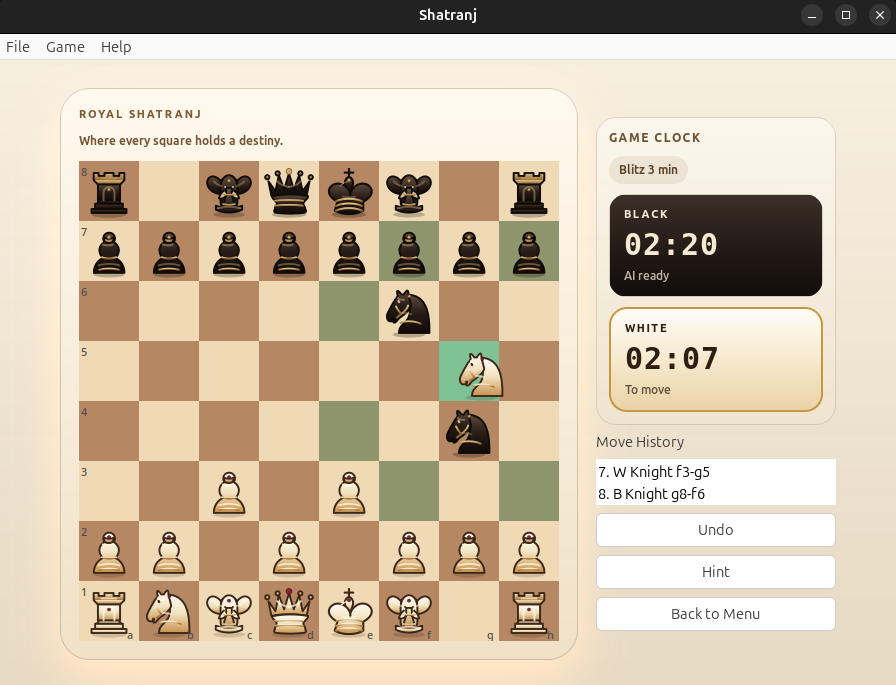
\includegraphics[width=0.75\textwidth]{GUI_SCREENSHOT_DRAG.png}}
  \caption{Drag-and-drop avec surbrillance des coups légaux}
  \label{fig:gui_drag}
\end{figure}

\subsection{Thread IA et synchronisation GTK}

Lancer l'IA dans le thread GTK principal bloquerait l'interface. Nous
utilisons un thread Python dédié et \texttt{GLib.idle\_add} pour
repasser dans le thread GTK principal avant toute modification d'état~:

\begin{minted}[frame=single,fontsize=\small]{python}
def _auto_play_ai_turns(self) -> None:
    def ai_thread():
            while (
                self._state is not None
                and self._state.current_color in self._ai_players
            ):
                if self._game_paused:
                    time.sleep(0.05)
                    continue
                ai = self._ai_players[self._state.current_color]
                move = ai.choose_move(self._state.board)
                if move is None:
                    break
                while self._game_paused and self._state is not None:
                    time.sleep(0.05)
                if (
                    self._state is None
                    or self._state.current_color not in self._ai_players
                ):
                    break
                # GLib.idle_add ensures GTK updates happen in the main thread
                done_event = threading.Event()
                GLib.idle_add(self._apply_ai_move, move, done_event)
                done_event.wait(timeout=5)
        thread = threading.Thread(target=ai_thread, daemon=True)
        thread.start()
\end{minted}

\texttt{done\_event} est un \texttt{threading.Event} qui synchronise le thread
IA avec le thread GTK~: l'IA ne calcule le coup suivant qu'une fois le coup
précédent appliqué et affiché.

\subsection{Horloge intégrée et CSS}

L'horloge est implémentée avec \texttt{GLib.timeout\_add(200, \_on\_timer\_tick)}~:
un tick toutes les 200~ms raffraîchit les labels. L'apparence est entièrement
définie en CSS (variable \texttt{CLOCK\_CSS})~: chaque carte horloge
(\texttt{clock-card-white}, \texttt{clock-card-black}) a son propre
dégradé. La classe \texttt{clock-card-active} ajoute un cadre doré
(\texttt{border: 2px solid \#c7963e}) sur la carte du joueur dont c'est le
tour, et
\texttt{clock-card-critical} passe le texte en rouge quand
il reste moins de 20~secondes.

Le dialogue de configuration propose quatre modes de contrôle du temps~:
Bullet, Blitz, Rapid et Custom. Le mode Custom utilise deux
\texttt{Gtk.SpinButton} (minutes et incrément) reliés à
\texttt{\_on\_custom\_time\_changed}~; le bouton ``Start Match'' ne devient
actif que quand un preset ou une valeur custom est sélectionnée.

\begin{figure}[H]
  \centering
  \fbox{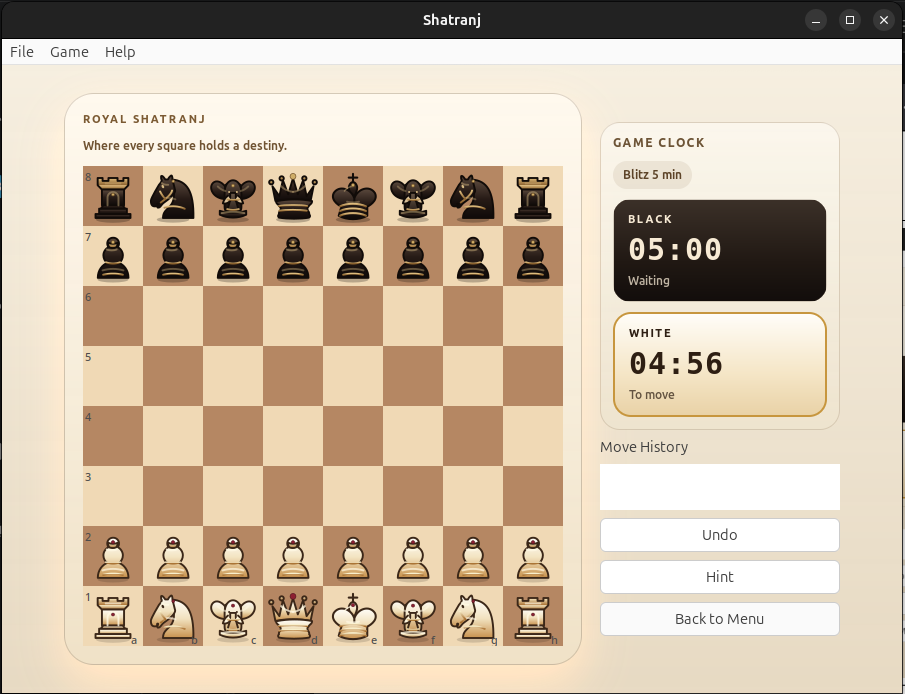
\includegraphics[width=0.75\textwidth]{GUI_SCREENSHOT_AI.png}}
  \caption{Horloge en mode blitz avec cartes White/Black}
  \label{fig:gui_clock}
\end{figure}

\subsection{Astuces et découvertes techniques}

\paragraph{Sauvegarde et chargement via le module \texttt{persistence}.}
Le GUI utilise directement les fonctions \texttt{load\_game\_file} et
\texttt{save\_game\_file} du module \texttt{shatranj/persistence.py},
qui encapsulent la sérialisation complète de l'état (plateau, horloge,
historique, configuration IA) au format ASCII structuré. Cette approche
garantit un format de fichier identique entre CLI et GUI sans duplication
de logique.

\paragraph{Conversion coordonnées pixel $\to$ case.}
Le plateau est redimensionnable. La conversion utilise \texttt{\_board\_geometry}~:
\[
  \text{col} = \left\lfloor \frac{x - \text{offset}_x}{\text{sq}} \right\rfloor,
  \quad
  \text{row} = 7 - \left\lfloor \frac{y - \text{offset}_y}{\text{sq}} \right\rfloor
\]
Le facteur $7 -$ est indispensable~: GTK mesure $y$ depuis le haut de la
fenêtre, alors que le Shatranj numérote les rangées depuis le bas.

\paragraph{Désactivation de l'interaction pendant le tour de l'IA.}
La méthode \texttt{set\_interaction\_enabled(False)} est appelée dès que
l'IA commence à réfléchir~: elle vide les états de sélection et de drag, et
ignore tous les événements souris. Cela évite les conditions de course entre
l'application d'un coup humain et le calcul de l'IA dans le thread secondaire.

%==============================================================================
\section{Revue critique du projet}
\label{sec:critique}
%==============================================================================

\subsection{Ce qui n'a pas été réalisé}

\begin{itemize}[noitemsep]
  
  \item \textbf{Machine Learning~:} l'intégration de Keras pour remplacer
    la sélection UCT dans le MCTS n'a pas été développée. Cette approche
    nécessite un corpus de parties de Shatranj de qualité pour l'entraînement~;
    or, contrairement aux échecs modernes qui disposent de millions de parties
    annotées (bases Lichess, ChessBase), le Shatranj est un jeu ancien dont
    les parties enregistrées sont rarissimes. Générer nous-mêmes ce corpus
    par auto-jeu aurait requis plusieurs jours de calcul, incompatibles avec
    les délais du projet.
\end{itemize}

\subsection{Performances}

L'AlphaBeta à profondeur~4 répond en moins de cinq secondes sur des positions
ouvertes. L'Iterative Deepening avec une limite de 5~secondes est plus robuste
en fin de partie~: il explore plus profondément quand le facteur de branchement
diminue. La table de transposition réduit le nombre de nœuds évalués de 30 à 50\,\%
sur les positions transposées au sein d'une même recherche. Le MCTS avec 500~simulations offre
une variété de jeu intéressante mais est plus lent~: environ 2~à~3~secondes par
coup en position ouverte.

\subsection{Cas limites et bugs identifiés}

\begin{itemize}[noitemsep]
  \item \textbf{Bug flag TT dans AlphaBeta~:} voir section~\ref{sec:_alphabeta}.
  \item \textbf{Pat dans le MCTS~:} le rollout traite le pat comme nul ($0{,}5$)
    plutôt que comme une défaite pour le joueur bloqué, ce qui sous-estime
    la valeur de forcer le pat contre l'adversaire.
  \item \textbf{TT vidée entre les itérations ID~:} \texttt{best\_move} appelle
    \texttt{self.\_tt.clear()} à chaque profondeur, annulant l'ordonnancement
    inter-profondeur théoriquement attendu.
    \item \textbf{Clé Zobrist figée dans le rollout MCTS~:}
    dans \texttt{\_rollout}, la clé de hachage est calculée une seule fois
    avant la boucle de simulation via
    \texttt{self.\_hasher.compute\_key(board, color)},
    puis n'est plus mise à jour après chaque coup joué
    (\texttt{board.apply\_move(move)}).
    Les résultats sont donc stockés dans la table de transposition
    sous la clé de la position \emph{initiale} du rollout,
    et non sous celle de la position terminale.
    Cela réduit l'efficacité du cache sans affecter la correction
    du résultat retourné.
\end{itemize}

\subsection{Améliorations possibles}

\begin{itemize}[noitemsep]
  \item Conserver la table de transposition entre les itérations de
    l'Iterative Deepening pour bénéficier de l'ordonnancement des coups.
  \item Corriger le traitement du pat dans le rollout MCTS pour qu'il
    corresponde aux règles officielles du Shatranj.
  \item Ajouter des benchmarks de performance pour mesurer le nombre de
    nœuds explorés et le temps de réponse moyen à profondeur~4.
    \item Mettre à jour la clé Zobrist de manière incrémentale à chaque coup
    joué dans \texttt{\_rollout} via \texttt{update\_key()},
    afin que chaque position simulée soit correctement indexée
    dans la table de transposition.
\end{itemize}

%==============================================================================
\bibliographystyle{plain}
\bibliography{bibliography}
%==============================================================================

%==============================================================================
\appendix
%==============================================================================

\section{Bilan des fonctionnalités (F1--F40)}
\label{sec:bilan}

\small
\renewcommand{\arraystretch}{1.2}

\begin{longtable}{>{\ttfamily}l p{8cm} c}
\caption{Bilan des fonctionnalités (F1--F40)} \\
\toprule
\textbf{ID} & \textbf{Description} & \textbf{État} \\
\midrule
\endfirsthead

\toprule
\textbf{ID} & \textbf{Description} & \textbf{État} \\
\midrule
\endhead

\midrule
\multicolumn{3}{r}{\textit{Suite page suivante}} \\
\endfoot

\bottomrule
\endlastfoot

\multicolumn{3}{l}{\textbf{Lancement et configuration}} \\
F1  & Options \texttt{-h}, \texttt{-V}, \texttt{-v}, \texttt{-d} & Fait \\
F2  & Fichier de configuration \texttt{.shatranjrc} & Fait \\
F3  & Internationalisation fr/en via \texttt{gettext} & Fait \\

\midrule
\multicolumn{3}{l}{\textbf{Options au lancement}} \\
F4  & Interface CLI par défaut & Fait \\
F5  & Mode Blitz avec chronomètre & Fait \\
F6  & Mode Contest (entrée fichier, sortie stdout) & Fait \\
F7  & Interface graphique GTK (\texttt{-g}) & Fait \\
F8  & Mode IA joueur (\texttt{-a W/B/A}) & Partiel \\

\midrule
\multicolumn{3}{l}{\textbf{Gestion du jeu}} \\
F9  & Validation des coups et mise à jour de l'état & Fait \\
F10 & Gestion des erreurs utilisateur (messages stderr) & Partiel \\
F11 & Undo / Redo & Fait \\
F12 & Hints (suggestion de coup via IA) & Fait \\
F13 & Blitz : décompte, pause, timeout & Fait \\

\midrule
\multicolumn{3}{l}{\textbf{Interface CLI}} \\
F14 & Shell interactif avec prompt \texttt{>>} & Fait \\
F15 & Proposition de sauvegarde avant de quitter & Fait \\
F16 & Édition de la ligne de commande (\texttt{readline}) & Fait \\
F17 & Historique des commandes (flèches, Ctrl+R) & Fait \\
F18 & Complétion Tab & partiel \\
F19 & Notation algébrique des coups & Fait \\

\midrule
\multicolumn{3}{l}{\textbf{Format de sauvegarde}} \\
F20 & Sauvegarde / restauration d'une partie & Fait \\
F21 & Commentaires dans la sauvegarde (\texttt{\#}, \texttt{\{\}}) & Fait \\
F23 & Format du plateau dans \texttt{[game]} & Fait \\
F24 & Format de l'historique dans \texttt{[history]} & Fait \\

\midrule
\multicolumn{3}{l}{\textbf{Bitboards}} \\
F25 & Module bitboard (primitives bit-à-bit) & Fait \\
F26 & Génération et application des coups & Fait \\

\midrule
\multicolumn{3}{l}{\textbf{Interface graphique}} \\
F27 & Menus File / Game & Fait \\
F28 & Raccourcis clavier & Fait \\
F29 & Drag-and-Drop & Fait \\

\midrule
\multicolumn{3}{l}{\textbf{Intelligence artificielle}} \\
F30 & Temps de réflexion borné & Fait \\
F31 & Minimax avec élagage $\alpha$-$\beta$ & Fait \\
F32 & Fonctions d'évaluation (material, positional, advanced) & Fait \\
F33 & Approfondissement itératif & Fait \\
F34 & Profondeur de recherche configurable & Fait \\
F35 & Monte Carlo Tree Search (MCTS) & Fait \\
F36 & Sélection par Machine Learning (Keras) & Non fait \\
F37 & Tables de transposition (Zobrist) & Partiel \\

\midrule
\multicolumn{3}{l}{\textbf{Jeu en réseau}} \\
F38 & Découverte de serveurs (UDP) et connexion TCP & Partiel \\
F39 & Serveur multi-clients, tableau des scores & Partiel \\
F40 & Système d'invitations, statuts des joueurs & Partiel \\

\end{longtable}

\section{Valeurs des pièces}
\label{sec:annexe-valeurs}

\begin{center}
\begin{tabular}{lcc}
\toprule
\textbf{Pièce} & \textbf{Valeur} & \textbf{Commentaire} \\
\midrule
Pion (Pawn)       & 1  & unité de base \\
Alfil             & 2  & 8~cases fixes de même couleur \\
Ferz              & 2  & 1~case en diagonale seulement \\
Cavalier (Knight) & 6  & saut en L, très mobile \\
Tour (Rook)       & 9  & ligne droite illimitée \\
Shah (Roi)        & 0  & non capturé, à protéger \\
\bottomrule
\end{tabular}
\end{center}

\end{document}